\documentclass[aspectratio=169,10pt]{beamer}

% Theme and typography
\usetheme{default}
\usecolortheme{default}
\setbeamertemplate{navigation symbols}{}

\usepackage{xcolor}
\definecolor{Navy}{HTML}{0F2042}
\definecolor{NavyLight}{HTML}{1E3A8A}
\definecolor{CyanAccent}{HTML}{0284C7}
\definecolor{SlateDark}{HTML}{1E293B}
\definecolor{SlateMuted}{HTML}{64748B}
\definecolor{LightBg}{HTML}{F8FAFC}
\definecolor{BorderCol}{HTML}{CBD5E1}
\definecolor{AlertRed}{HTML}{DC2626}
\definecolor{SuccessGreen}{HTML}{059669}

\setbeamercolor{frametitle}{fg=Navy,bg=white}
\setbeamercolor{title}{fg=Navy}
\setbeamercolor{structure}{fg=NavyLight}
\setbeamercolor{normal text}{fg=SlateDark}

\setbeamertemplate{footline}{
  \leavevmode%
  \hbox{%
    \begin{beamercolorbox}[wd=.85\paperwidth,ht=2.5ex,dp=1.1ex,leftskip=1cm]{normal text}%
      \fontsize{7.5}{9}\selectfont\color{SlateMuted}2026 Carnegie Mellon Forum on Biomedical Engineering \enspace$\cdot$\enspace Abstract \#194 Poster Summary
    \end{beamercolorbox}%
    \begin{beamercolorbox}[wd=.15\paperwidth,ht=2.5ex,dp=1.1ex,rightskip=1cm]{normal text}%
      \fontsize{7.5}{9}\selectfont\bfseries\color{NavyLight}Slide \insertframenumber{} of 3
    \end{beamercolorbox}%
  }%
  \vskip2pt%
}

\usepackage{graphicx}
\usepackage{booktabs}
\usepackage{tcolorbox}
\tcbuselibrary{skins}

\tcbset{
  cardstyle/.style={
    enhanced, colback=LightBg, colframe=BorderCol, boxrule=1pt, arc=2mm,
    left=3.5mm, right=3.5mm, top=2.5mm, bottom=2.5mm
  }
}

\begin{document}

% =========================================================================
% SLIDE 1: Title, Authors, Background, Purpose of the Study
% =========================================================================
\begin{frame}[t]{Discrete Latent Sequence Generation for 12-Lead ECG Reconstruction}
  \vspace{-0.7em}
  % Author & Affiliation Banner with Logos
  \begin{tcolorbox}[cardstyle,colframe=CyanAccent,top=0.6mm,bottom=0.6mm,left=1.5mm,right=1.5mm]
    \begin{columns}[c]
      \begin{column}{0.19\textwidth}
        \centering
        
\includegraphics[height=0.50cm,keepaspectratio]{figures/compressed/logos/uoft_cs_logo.png}
      \end{column}
      \begin{column}{0.60\textwidth}
        \centering
        \fontsize{7.5}{9}\selectfont
        \textbf{\color{Navy}Mithun Manivannan, BSc}$^{1}$ \enspace \textbf{Alex Mariakakis, PhD}$^{1}$ \enspace \textbf{Christopher Cheung, MD}$^{2}$\\[0.5pt]
        \fontsize{6}{7.2}\selectfont\color{SlateDark}
        $^{1}$Department of Computer Science, University of Toronto \quad $^{2}$Division of Cardiology, Sunnybrook Health Sciences Centre\\[0.5pt]
        \color{CyanAccent}\textbf{Carnegie Mellon Forum on Biomedical Engineering 2026 \enspace$\cdot$\enspace Abstract Submission \#194}
      \end{column}
      \begin{column}{0.19\textwidth}
        \centering
        
\includegraphics[height=0.50cm,keepaspectratio]{figures/compressed/logos/sunnybrook_logo.png}
      \end{column}
    \end{columns}
  \end{tcolorbox}

  \vspace{-2pt}
  \begin{columns}[T]
    \begin{column}{0.49\textwidth}
      \begin{tcolorbox}[cardstyle,colframe=NavyLight,top=1mm,bottom=1mm,left=2mm,right=2mm,title={\bfseries\fontsize{7.5}{9}\selectfont\color{Navy}Clinical Background \& Motivation}]
        \fontsize{6.2}{7.4}\selectfont
        \begin{itemize}\setlength{\itemsep}{0.5pt}\setlength{\parskip}{0pt}\setlength{\leftskip}{-10pt}
          \item \textbf{12-Lead Gold Standard}: Standard clinical cardiology relies on 10 electrodes capturing 3D cardiac electrical dipoles across frontal and horizontal planes, critical for diagnosing myocardial infarction, ischemia, and chamber hypertrophy.
          \item \textbf{Ambulatory Wearable Reality}: Consumer smartwatches (Lead I) and patch monitors (Lead II) provide continuous at-home monitoring but are blind to 10 of 12 spatial vectors.
          \item \textbf{The Inverse Problem}: Reconstructing 12 leads from limited leads is mathematically ill-posed; infinitely many 3D dipoles project to identical 1D traces.
          \item \textbf{Failure of MSE Regression}: Point-wise $L_2$ loss causes regression-to-the-mean, amplitude damping, and severe distortion of local clinical fiducials (QRS, ST, QT).
        \end{itemize}
      \end{tcolorbox}
    \end{column}
    \begin{column}{0.49\textwidth}
      \begin{tcolorbox}[cardstyle,colframe=SuccessGreen,top=1mm,bottom=1mm,left=2mm,right=2mm,title={\bfseries\fontsize{7.5}{9}\selectfont\color{SuccessGreen}Purpose of the Study}]
        \fontsize{6.2}{7.4}\selectfont
        \begin{itemize}\setlength{\itemsep}{0.5pt}\setlength{\parskip}{0pt}\setlength{\leftskip}{-10pt}
          \item \textbf{Novel Generative Framework}: Formulate \textbf{ECG-AIM}, a discrete latent sequence generation framework combining multi-resolution Morlet wavelets with spatiotemporal axial attention to reconstruct 12 leads from limited inputs.
          \item \textbf{Factorial $2^4$ Loss Benchmarking}: Systematically dissect amplitude, correlation, distribution, and slope constraints across 3 paradigms (U-Net, MultiScale-VAE, ECG-AIM).
          \item \textbf{Physical Prior Enforcement}: Integrate Kirchhoff limb conservation ($\text{I} + \text{III} = \text{II}$) to ground frontal plane geometry.
          \item \textbf{Clinical \& Hardware Validation}: Audit sub-10ms fiducial accuracy, downstream structural heart disease preservation, and zero-shot hospital cart transfer.
        \end{itemize}
      \end{tcolorbox}
    \end{column}
  \end{columns}
\end{frame}

% =========================================================================
% SLIDE 2: Methods
% =========================================================================
\begin{frame}{Methods: Architecture, Multi-Objective Loss \& Training Pipeline}
  \vspace{-0.5em}
  \begin{columns}[T]
    \begin{column}{0.54\textwidth}
      \centering
      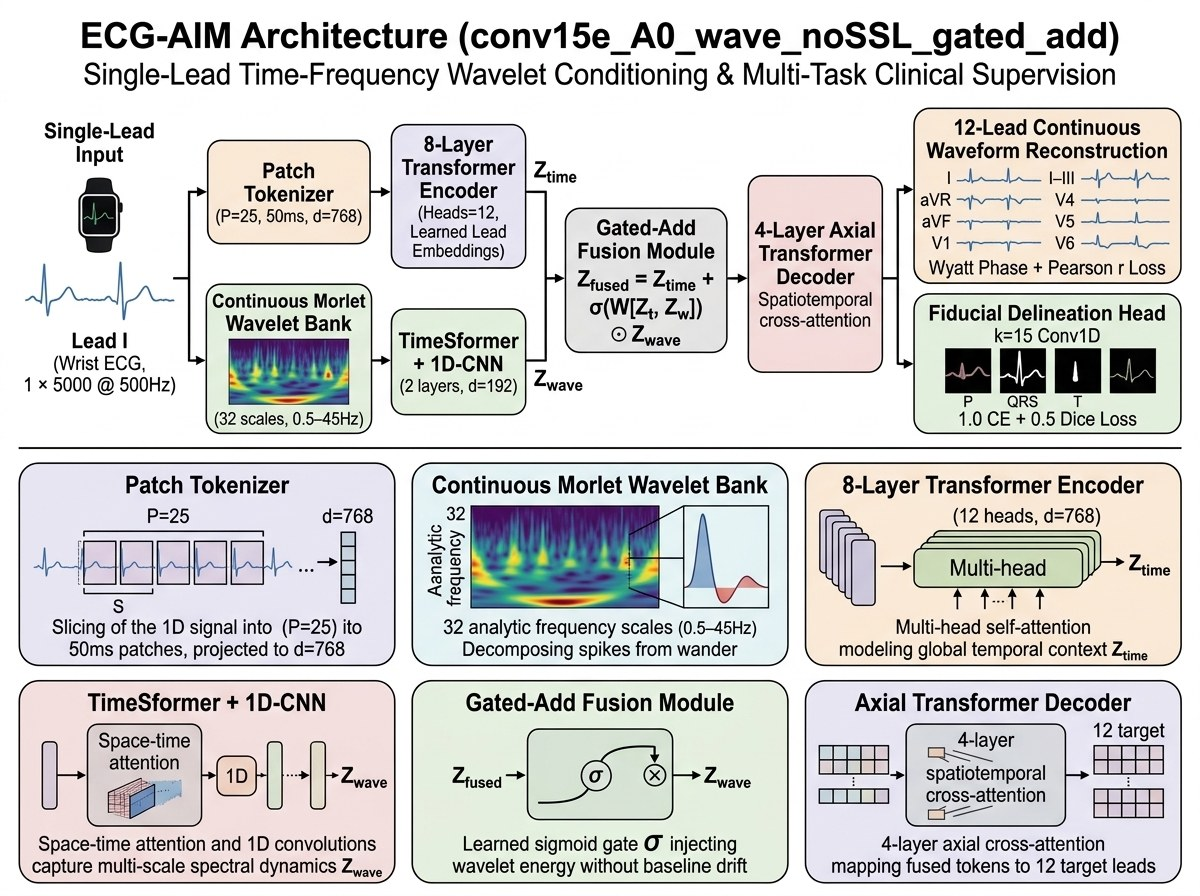
\includegraphics[width=\linewidth,height=0.38\textheight,keepaspectratio]{figures/compressed/conv15e_a0_wave_architecture.jpg}\\[2pt]
      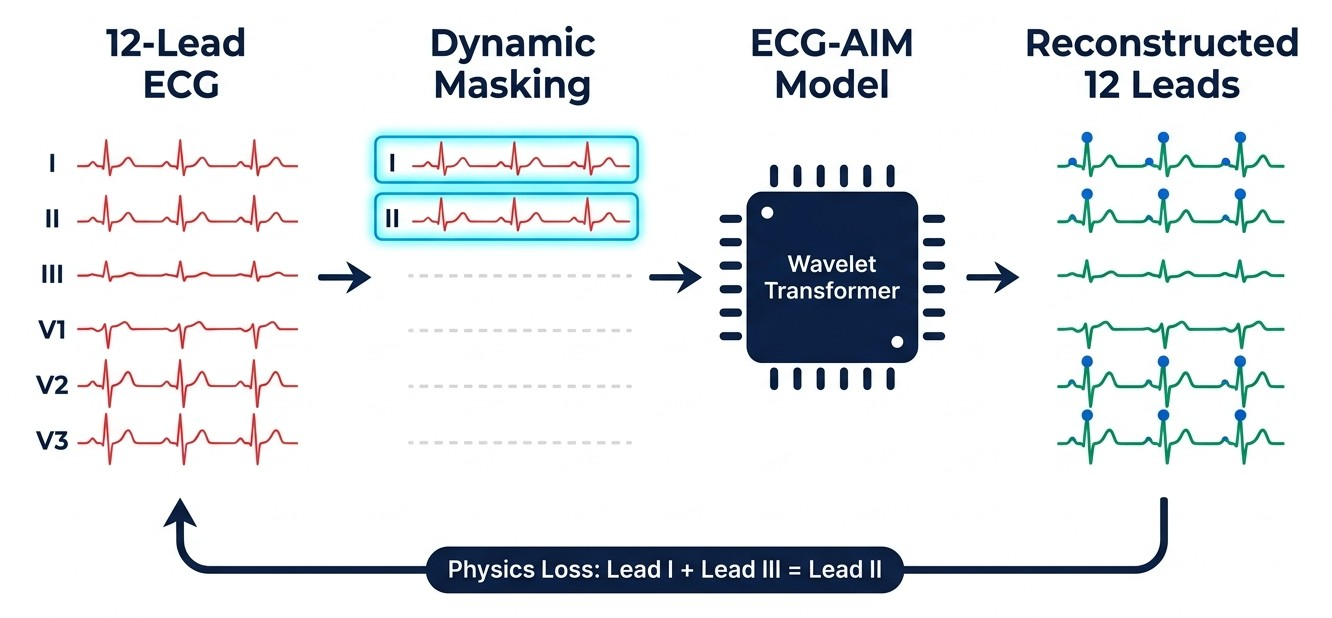
\includegraphics[width=\linewidth,height=0.34\textheight,keepaspectratio]{figures/compressed/ecg_aim_training_pipeline.jpg}
    \end{column}
    \begin{column}{0.44\textwidth}
      \begin{tcolorbox}[cardstyle,colframe=NavyLight,title={\bfseries\color{Navy}1. Dual-Branch Model Architecture}]
        \fontsize{7}{8.8}\selectfont
        \textbf{Patch Tokenizer}: 50 ms patches mapped to $d=768$ temporal tokens via an 8-layer Transformer encoder.\\
        \textbf{Morlet Wavelet Bank}: 32 analytic scales (0.5--45 Hz) extracts multi-resolution time-frequency scalograms.\\
        \textbf{Gated-Add Fusion}: $Z_{\text{fused}} = Z_{\text{time}} + \sigma(W[Z_t, Z_w]) \odot \text{Proj}(Z_w)$.\\
        \textbf{Axial Decoder}: Spatiotemporal cross-attention predicting 12-lead waveforms and explicit P-QRS-T masks.
      \end{tcolorbox}
      \vskip 1pt
      \begin{tcolorbox}[cardstyle,colframe=SuccessGreen,title={\bfseries\color{SuccessGreen}2. Factorial Multi-Objective Loss}]
        \fontsize{7}{8.8}\selectfont
        $\mathcal{L} = \mathcal{L}_{\text{MSE}} + 0.5\mathcal{L}_{\text{corr}} + 0.1\mathcal{L}_{\text{MMD}} + 0.05\mathcal{L}_{\Delta} + \lambda\mathcal{L}_{\text{limb}}$\\
        \textbf{Kirchhoff Limb Prior}: $\mathcal{L}_{\text{limb}} = \|\hat{y}_{\text{II}} - (\hat{y}_{\text{I}} + \hat{y}_{\text{III}})\|_2^2$ eliminates frontal vector drift.
      \end{tcolorbox}
      \vskip 1pt
      \begin{tcolorbox}[cardstyle,colframe=CyanAccent,title={\bfseries\color{CyanAccent}3. Large-Scale Multi-Task Pretraining}]
        \fontsize{7}{8.8}\selectfont
        Trained on 175,890 observations (PTB-XL \& MIMIC-IV) with dynamic lead masking ($M_{\text{obs}}$) accepting 1-lead to 3-lead inputs.
      \end{tcolorbox}
    \end{column}
  \end{columns}
\end{frame}

% =========================================================================
% SLIDE 3: Results and Conclusion
% =========================================================================
\begin{frame}{Results and Conclusion: Clinical Precision \& Hardware Translation}
  \vspace{-0.5em}
  \begin{columns}[T]
    \begin{column}{0.54\textwidth}
      \centering
      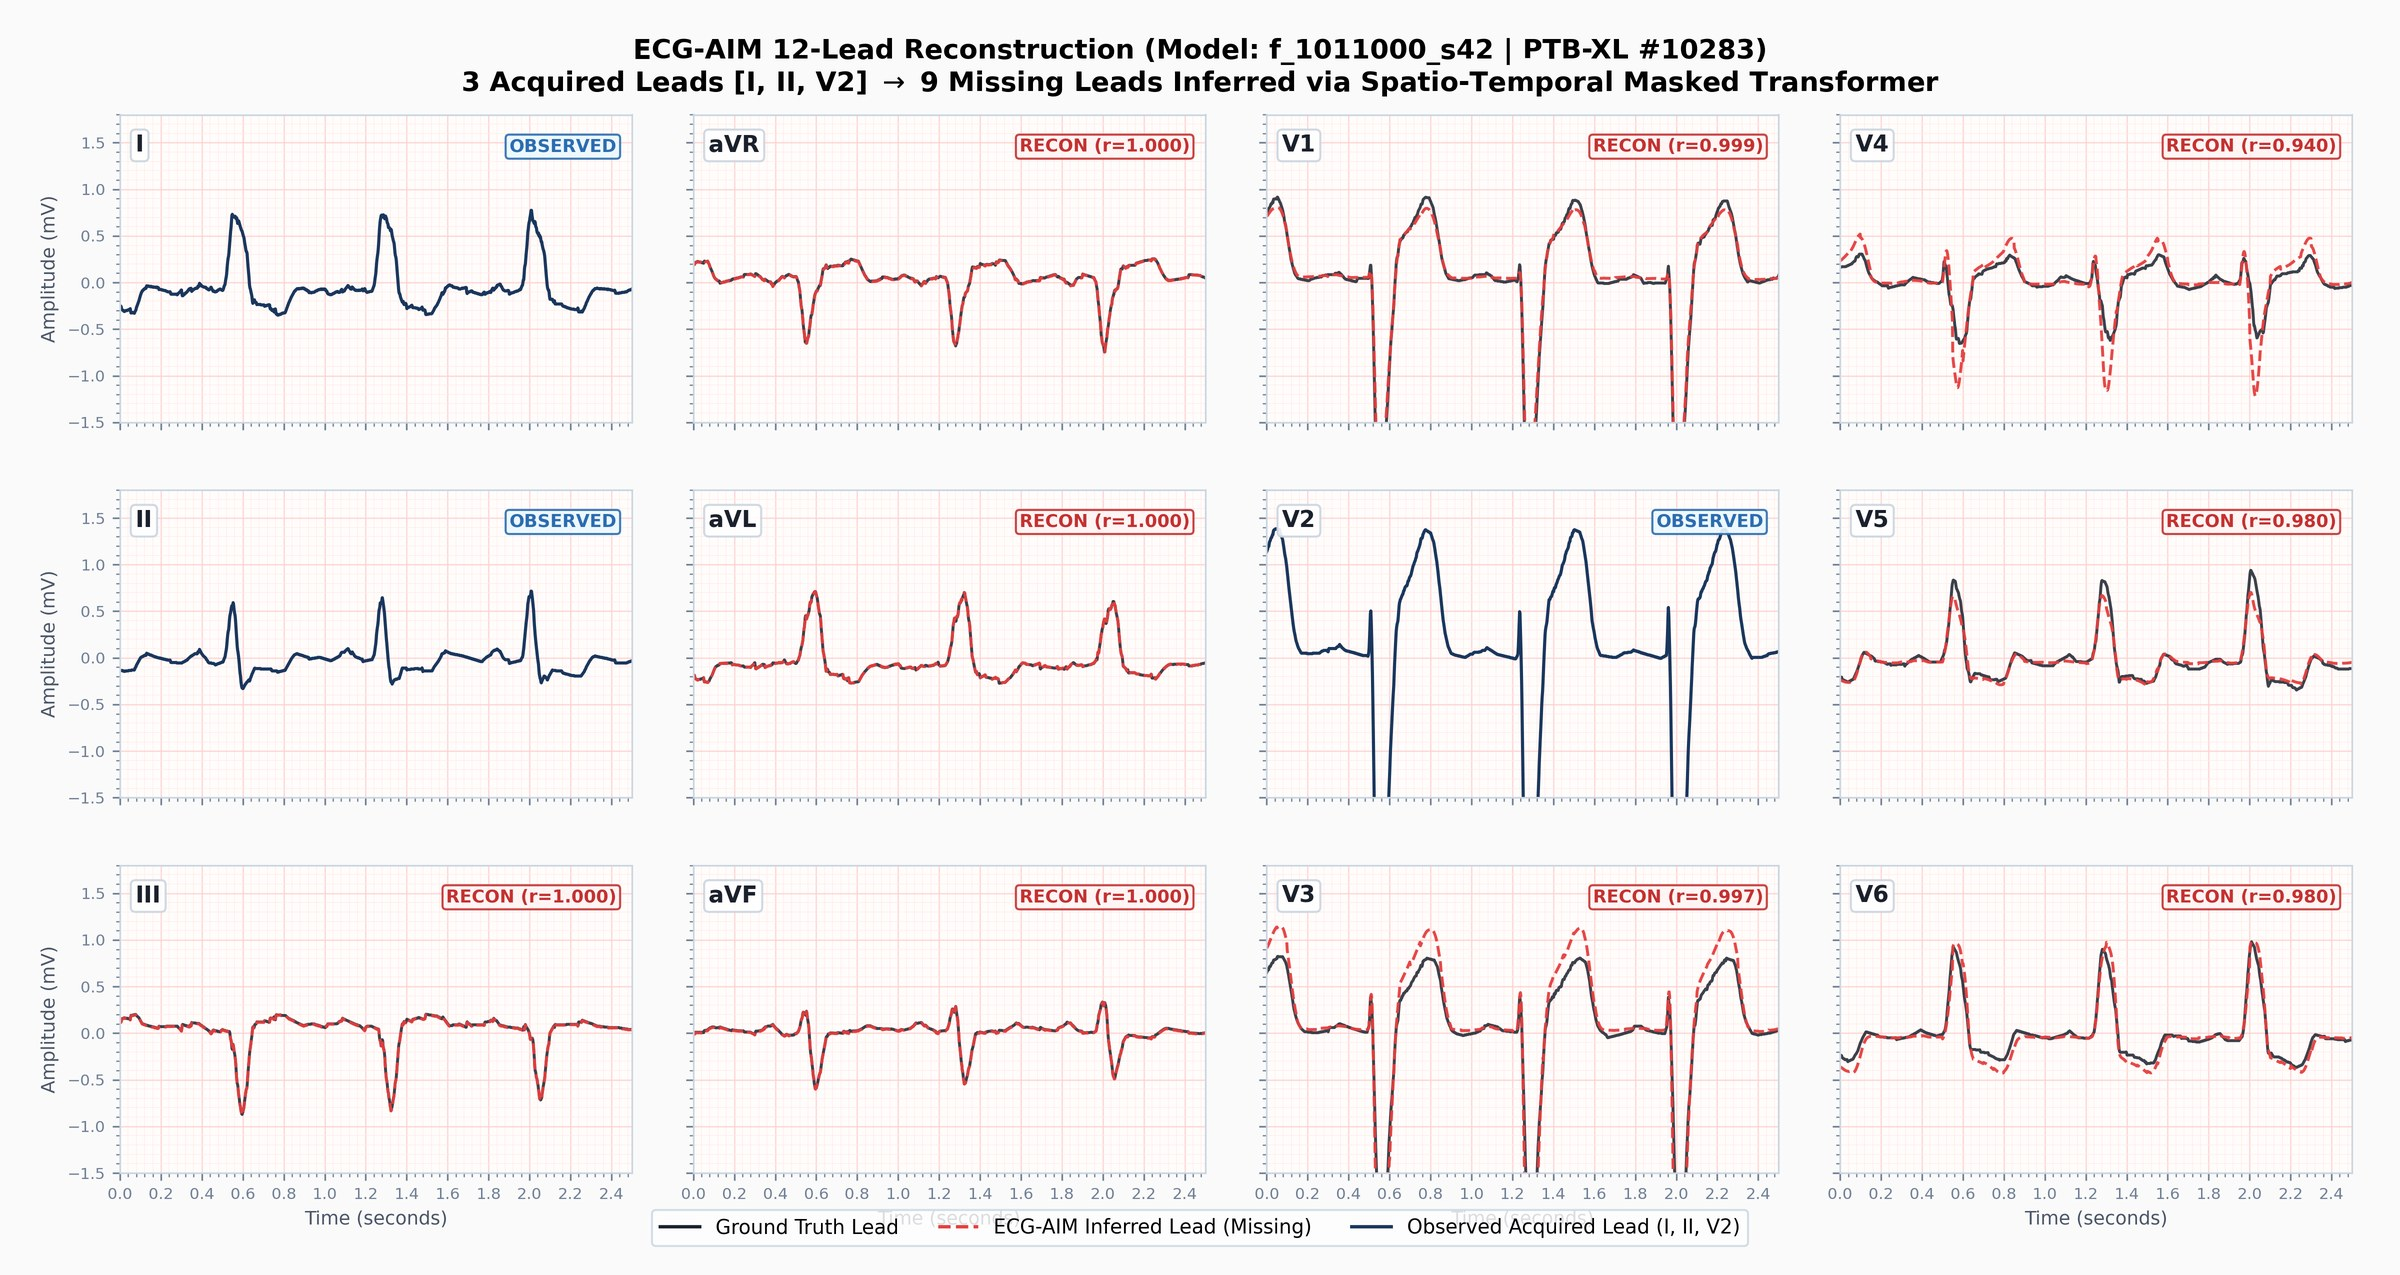
\includegraphics[width=\linewidth,height=0.46\textheight,keepaspectratio]{figures/compressed/best_ecg_aim_12lead_reconstruction.jpg}
      \vskip 2pt
      % Compact table
      \resizebox{\linewidth}{!}{%
      \begin{tabular}{lcccc}
        \toprule
        \textbf{Endpoint Dimension} & \textbf{Baseline U-Net} & \textbf{Stanford 3DRECON} & \textbf{ECG-AIM (Ours)} & \textbf{Clinical Impact} \\
        \midrule
        Precordial Chest Mean $r$ & 0.570 & 0.732 & \textbf{0.776} & $\Delta=+0.206$ ($p < 10^{-300}$) \\
        QRS Duration MAE & 13.85 ms & 10.26 ms & \textbf{8.0 ms (Median)} & Sub-10ms clinical gate \\
        Conduction Delay ($>$120ms) & 90.7\% & 94.3\% & \textbf{94.3\%} & aOR = 1.84 ($p < 10^{-17}$) \\
        Sokolow-Lyon LVH Voltage & 1.13 mV & 0.63 mV & \textbf{0.72 mV} & $r=0.714$ chamber concordance \\
        EchoNext Structural Disease & 68.8\% & \color{AlertRed}\textbf{46.5\% (Collapse)} & \color{SuccessGreen}\textbf{71.6\%} & Preserves echo pathology \\
        \bottomrule
      \end{tabular}%
      }
    \end{column}
    \begin{column}{0.44\textwidth}
      \begin{tcolorbox}[cardstyle,colframe=SuccessGreen,title={\bfseries\color{SuccessGreen}1. Near-Lossless 3-Lead Diagnostic Triad}]
        \fontsize{7.5}{9.5}\selectfont
        Leads I, II, and $V_2$ lock the 3 orthogonal dipoles ($X, Y, Z$), achieving precordial Pearson $r = \mathbf{0.980\text{--}1.000}$ and preserving anterior ST elevation.
      \end{tcolorbox}
      \vskip 2pt
      \begin{tcolorbox}[cardstyle,colframe=AlertRed,title={\bfseries\color{AlertRed}2. Overcoming Diagnostic Collapse}]
        \fontsize{7.5}{9.5}\selectfont
        Prior state-of-the-art (Stanford 3DRECON) collapsed to \textbf{46.5\%} on downstream EchoNext structural heart disease. ECG-AIM maintains \textbf{71.6\%} by preventing amplitude regression.
      \end{tcolorbox}
      \vskip 2pt
      \begin{tcolorbox}[cardstyle,colframe=Navy,title={\bfseries\color{Navy}3. Hospital Cart Hardware Validation}]
        \fontsize{7.5}{9.5}\selectfont
        Zero-shot testing on Sunnybrook physical 10-wire XML carts confirms authentic clinical voltages ($>$2.1 mV in $V_2$) while preserving the true 18 $\mu$V analog noise floor.
      \end{tcolorbox}
      \vskip 2pt
      \begin{tcolorbox}[cardstyle,colframe=CyanAccent,title={\bfseries\color{CyanAccent}4. Study Conclusion}]
        \fontsize{7.5}{9.5}\selectfont
        Discrete latent sequence generation with continuous wavelet fusion successfully enables diagnostic 12-lead reconstruction from limited leads.
      \end{tcolorbox}
    \end{column}
  \end{columns}
\end{frame}

\end{document}
